\setcounter{chapter}{1}
\chapter{Neuroanatomy}
\label{sec:neuro}
%
\note{\paragraph{Ziele:} 
\begin{itemize}
    \item uebersicht neuroanatomy
    \item struktureller aufbau nervenfaser
    \item ableitbare eigenschaften fuer modelle
\end{itemize}}
%
\section{Introduction}
% 
Neuroanatomie is the study of the structure of the brain.
Its task are to investigage the sizes, regions and structure of the nerve system in humans and animals.
This is a quite dificult task size the brain, especially the human brain, is one of the most complex organs with a large viarty of cells, connections, topography and the from this resulting functionalities.
With the development of the microscope and after the overcome of the concerns to experiment on dead human tissue, in the last few hundread years more and more of the structure of the human brain was descovered.
Recently techniques likee \acs{dMRI}, fluorescence microscopy, stained microscopy, autoradiography (too name only a few), were able to investigate more and more structures from different points of views in the brain with increasing resolution and on different species.
Different species help to understand the evolution of the brain. Additionally the brains of commenly rodens and apes are not as large and not as evolved as the human brain.
This helps to research structure which are not as complex as the human brain.
%
% 
% 
\section{Brain Architecture}
% 
\begin{figure}[!t]
\centering
\subcaptionbox{\label{fig:headAndBrain}}[.28\textwidth]{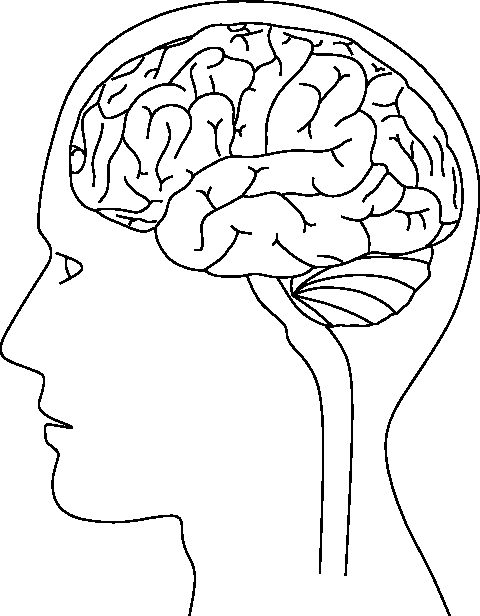
\includegraphics[height=3cm]{gfx/neuroanatomy/human-brain-profile.pdf}}
\subcaptionbox{}[.35\textwidth]{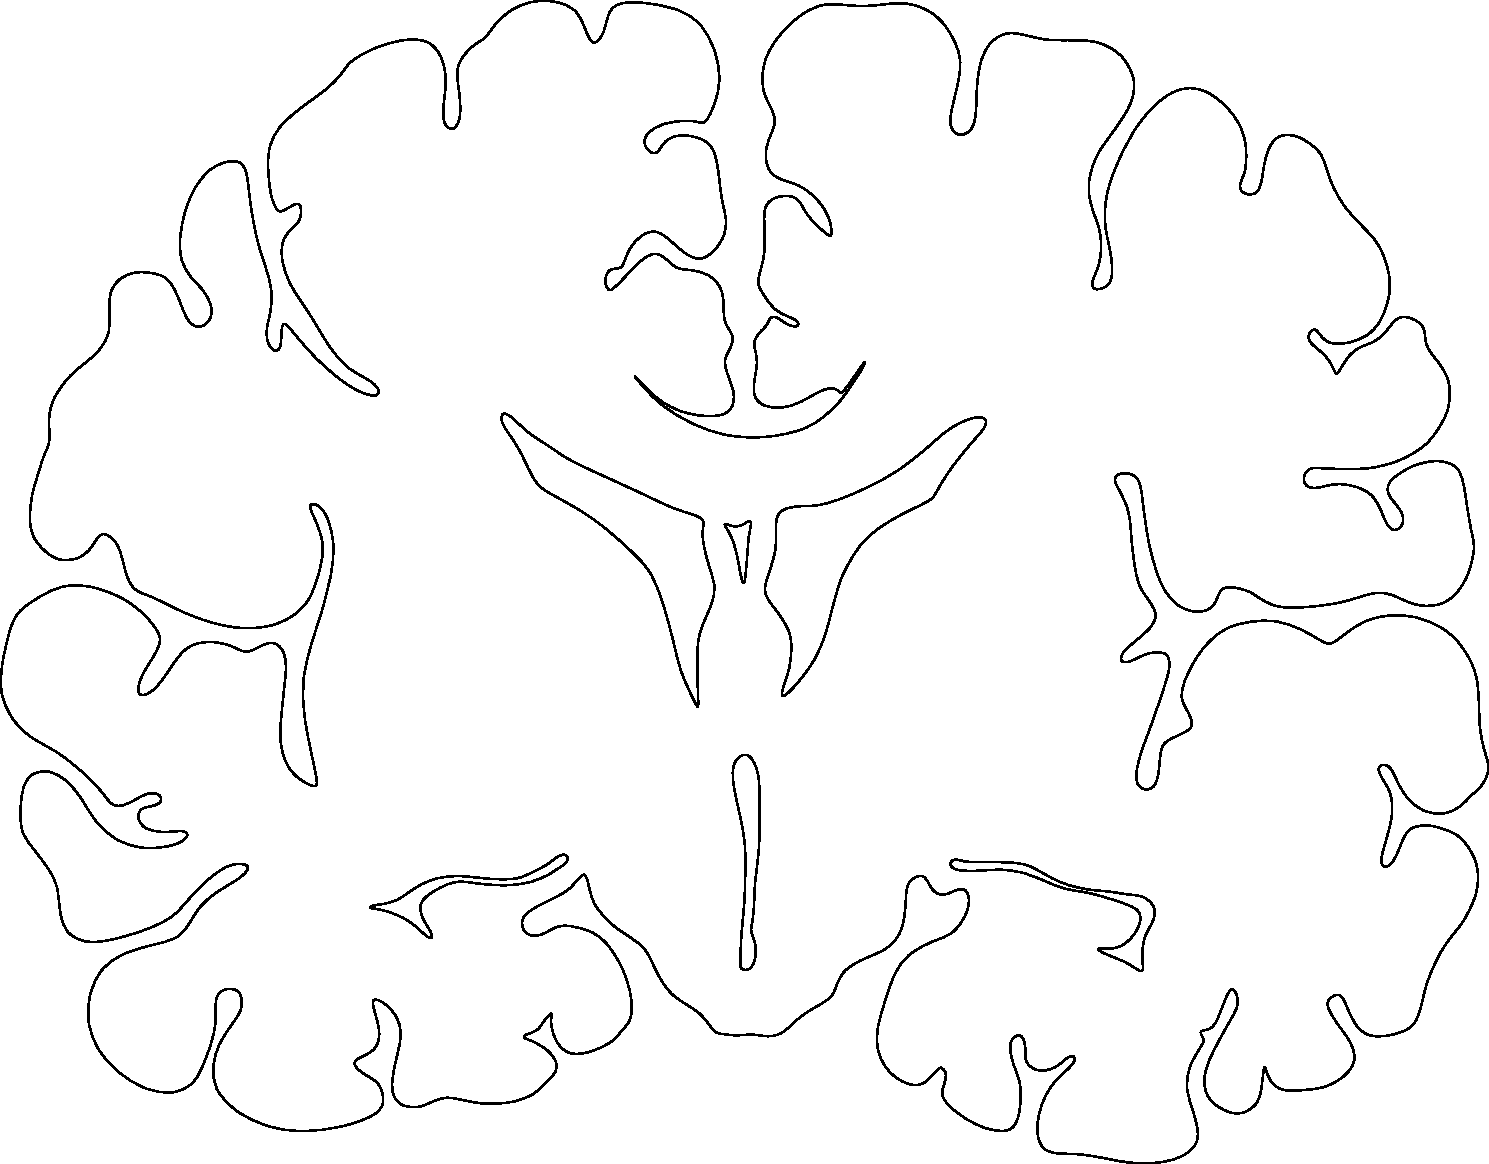
\includegraphics[height=3cm]{gfx/neuroanatomy/human-brain-section.pdf}}
\subcaptionbox{\label{fig:nerveFiber}}[.35\textwidth]{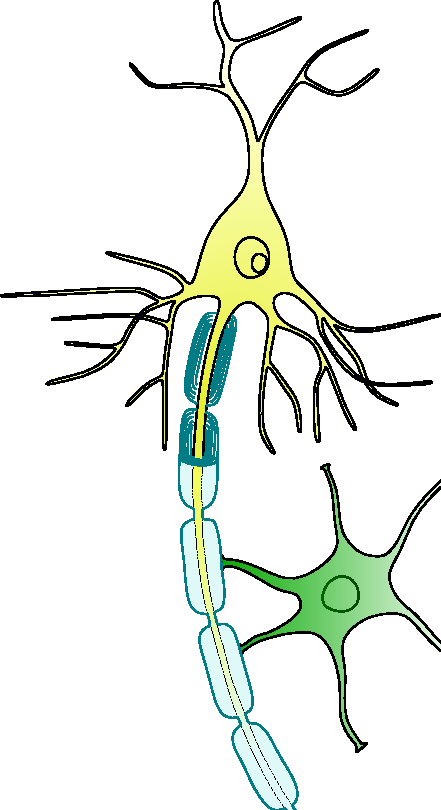
\includegraphics[height=3cm]{gfx/neuroanatomy/neuron-axon.pdf}}
\caption{(a) Illustration of human brain. (b) Illustration of a coronal human brain section. (c) Illustration of a neuron with axon and oligodendrocytes.}
\label{fig:human-brain}
\end{figure}
% 
The human brain (see \cref{fig:headAndBrain}) consist out of three major parts: the cerebellum, which is located at the rear bottom, the cerebrum, located at the top and the brainstem, which is underneath and connects the other parts of the brain with the spinal.
\\
The brainstem is the connection between the different brain areals and the spinal cord.
It can be further divided into the midbrain, the pons and medulla obiongata, which themself are further specialised.
\\
The cerebellum most important task in the human brain is the motor control.
It is highly folded which allows it to have an especially high surface area, which will be important in a later step.
\\
The cerebrum in the human brain is the biggest part.
If is folded as well and has a left and right hemisphere.
Additionally the cerebrum can be seperated into 4 visible parts, seperated by \dummy{} (\eg{} sulcus centralis.
% 
\begin{figure}[!t]
\centering
\hspace*{\fill}
\subcaptionbox{\label{fig:brainLobes}}[.45\textwidth]{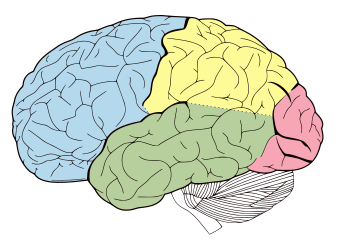
\includegraphics[height=3cm]{dev/wiki/brain_lobes.png}\url{https://en.wikipedia.org/wiki/Frontal_lobe}}
\hspace*{\fill}
\subcaptionbox{\label{fig:nerveFiber}}[.45\textwidth]{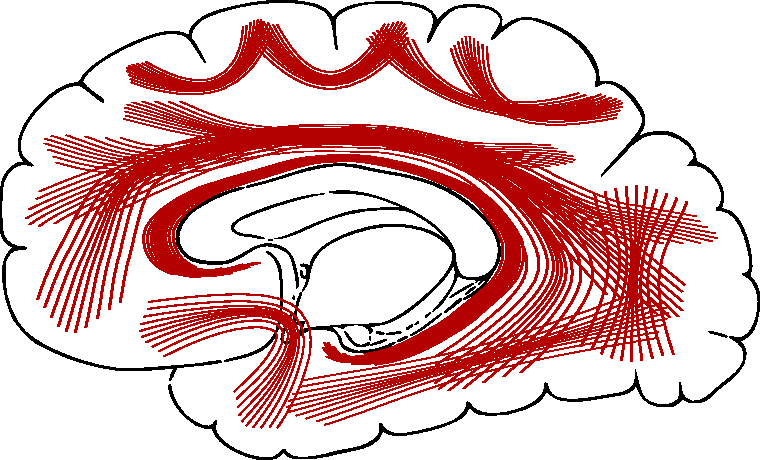
\includegraphics[height=3cm]{dev/wiki/brain_fiber_paths.png}\url{https://en.wikipedia.org/wiki/Association_fiber}}
\hspace*{\fill}
\caption{(a) Illustration of human brain. (b) Illustration of a coronal human brain section.}
\label{fig:human-fiber}
\end{figure}
% 
The frontal, parietal, temporal  and occipital lobe (see \cref{fig:brainLobes}).
\\
The frontal lobe contains most of the ... functionalities.
The parietal lobe has \dummy{}
The ocipital lobe main function is the signal processing of the visual system.
The temporal lobes contain visual memories as well es auditry functions and language.
\par
The inner part of the brain also include cortival(? -> gm) structures like \dummy{}.
All this structures in the cerebellum and the cerebum contain on thir surfaces (outer as well as inner) a cortical (?) layer, which is filled with cell bodies.
This cells purpase are to process the information of all the signals comming from outside (and inside) the brain.
There are many types of cells involed in this process.
For example some can strengthen a signal or inhibite it.
In the human brain there are several (Billion?) cells which have a high interconnectivity in the local area as well as through the brain to different ...
This high coplex structure is the source of human intelligence, consisnes and much more.
Therefore it is a common goal of humanity to understand the human brain to improve medical treatment as well as \dummy{}.
% 
\paragraph{Further information}
This is only a short introduction into the brain architecture.
It can be further seperated into much more objective parts as well as ...
This is for example done via cell types and density research like the investigation of cortical layers.
% 
% 
% 
\section{Fiber Architecture} \label{sec:fiberArchitecture}
% 
\begin{figure}[!t]
\centering
% 
\hspace*{\fill}
\tikzset{external/export next=false}
\subcaptionbox{\label{fig:coronalStained}BB 4201: Gray, White Matter, Coronal Section, Stained}[0.6\textwidth]{
\begin{tikzpicture}[]
    \node[inner sep=0pt, anchor = south west] (fig) at (0,0)
    {\includegraphics[width=0.6\textwidth]{dev/brain/BB_4201.png}};
    % \draw[] (0,0) grid (8,5);
    \draw[RED, ultra thick, <-] (5,4) -- ++ (-42:0.75) node[pos=1, anchor=north] {\textbf{WM}};
    \draw[GREEN, ultra thick, <-] (2.4,5) -- ++ (-65:0.75) node[pos=1, anchor=north] {\textbf{GM}};
\end{tikzpicture}
}
\hspace*{\fill}
\subcaptionbox{Cortical layers}[0.3\textwidth]{
\includegraphics[width=0.3\textwidth]{dev/wiki/layers.png}
}
\hspace*{\fill}
% 
\caption[GM, WM, layers]{}
\label{fig:BBrain}
\end{figure}
% 
Nerve cells are connected via different types of (nerve?) fibers.
A typical nerve cell (if there is such a thing) has a cell body, which processes the incomming information.
The information arives via dendrites, which are star like tree branches, which will connect to an incomming axon.
The axon is the main (and only) output of the cell.
It travels through the brain to its destination and connects there to a (maybe more or less random) brain cell.
This randomness is most likely also part of the learning process in child development, since after the brain axons are developed, no new axons are build anymore.
Only the strength of the signals and local structues changes as well as no used connections can be \say{deleted}.
Since there are (Billion?) of nerve cells, and there axons need ro reach a specific targed in a closed volume, the density of nerve fibers is quite high.
There diameter is around $\SI{0.5}{\micro\meter}$ up to several $\si{\micro\meter}$.
The axon is surrounded by a myelin sheet, which is a lipid layerd structure, build from near by olegodendrides.
These souroundings electic isolates the axon.
This improves the travelling speed of the electirc action potential along the axon as well as its signal strength (voltage).
There are many different types of axons.
Some contain a very thick layer of myelin while others have none.
The high density of Axons and myelin lets the inner part of the brain, where almost all axons are located, whithly looking
Therefore it has the name \ac{WM}.
The outer cell bodies layer are called \ac{GM}.
In a stained image this is visible (see \cref{fig:coronalStained}).
\par
% 
\begin{figure}[!t]
	\centering
	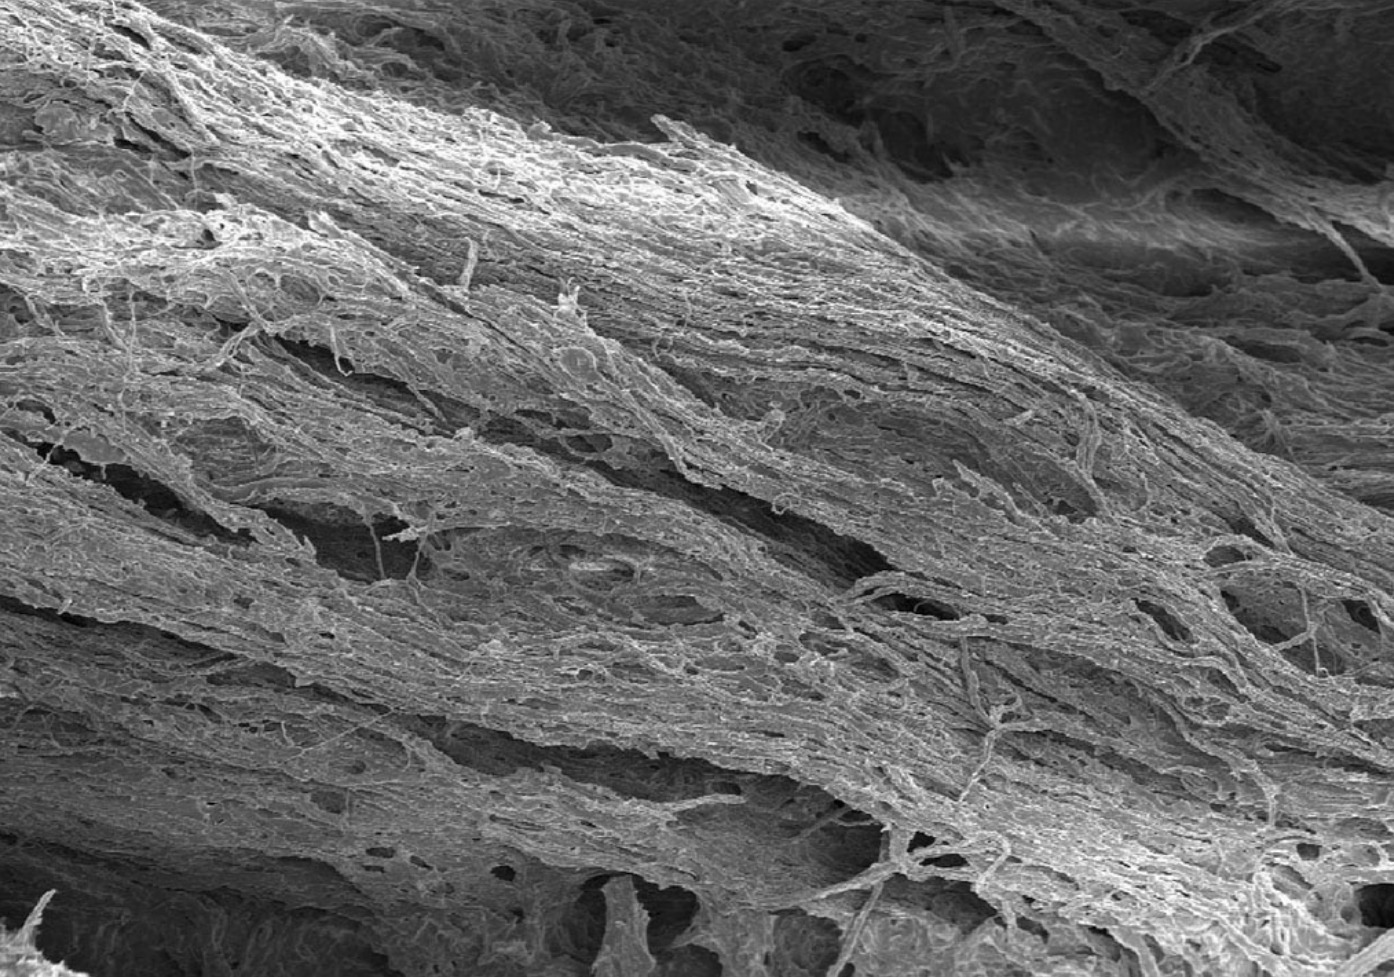
\includegraphics{gfx/neuroanatomy/human_wm_after_klinger_dissection.png}
	\caption{Electron microscopy image after klinger dissection \cite{destrieux:hal-01261930}.}
% 	\label{fig:brain_sectioning}
\end{figure}
% 
Since this \ac{WM} has such a high density of fibers (up to billion in the corpus calosum) it is even under a microscop nearly impossible to investigate single fiber trackts thorugh the brain.
For different species with smaller brains, like rodens, imaging techniques like \textit{clearing} have a high potential and could already been used to map an (entire?) brain with axons.
However for a more complex and larger brain, this is up to this point not achieved.
Polarized light imaging, which uses the birefringence property of myelin, is a promassing technique, already developed in the 1900, which allows to map the orientation of axons in a brain section.
This technique has, as all microscopic techniques wich are using sections, the disadvantage, that the brain has to be cut and measured afterwards.
There are alternative methods like (OCT?), which measures the brain section first, and then cuts the upper layer away, and mesures the next "section" afterwards. It uses the reflexion of the light than rather the transmittanted light thorugh the tissue.
However up to this point no entire large brain like a human brain was measured in its entirety.
Since \ac{3D-PLI} uses the already known sectioning techniques, which are developed since several decades, it can use this knowlege to its advantage.
% 
%
\section{Sectioning}
%
\begin{figure}[!t]
	\centering
    \def\tikzwidth{0.75\textwidth}
	\inputtikz{gfx/neuroanatomy/brain_sectioning}
	\caption{Illustration of sectioning.}
	\label{fig:brain_sectioning}
\end{figure}
% 
For the cutting process, the tissue, \ie{} the brain, has to be frozen and imbedded into a solid material.
One commen material is parafine, however this is not possible for \ac{3D-PLI} \dummy[why?]{}.
For \ac{3D-PLI} it very is important, that the tissue does not build up crystal structures, because these are also birefringence.
therefore the tissue is first ... into a ... liquid ...
After a time of a few months the tissue will then be frozen into a \SI{-70}{\degree}.
Then the frozen tissue can be fixated with a liquid glue on a cutting plate.
The glue is ...
It is also be used to build up a sourounding fixating material to stabilize the brain in the cutting process.
Additionally markers are fixed which help in the later registration process, which will align the tissue sections in a 3d volume again.
\par
The cutting is done in a microtome.
In there the temperature can be held at about \SI{-70}{\degree} and allows no heating of the tissue.
The brain is moved against a vibrating very sharp knife.
This allows for the thin sectioning of about \SI{60}{\micro\meter}.
After the cutting, the tissue is put onto a glass specimen.
Since the tissue is such thin and filigran, it is not always possible to avoid cracks for example.
This also will be as best as possible corrected in the registration process.
The tissue will be ... with a glycerin ... and finally siled with another glass.
To prevent the formation of waves in the tissue, the glass is weighted.
The tissue sections are then stored into a refrigerator at \SI{-70}{\degree\celsius}.
The tissue can then finally be measured in the \ac{3D-PLI} microscopes (see \cref{sec:expSetup} for further techniqule informations).
% 
% 
\section{Axon Literature}
\label{microscopy}
% 
Axon diameter \cite{Liewald2014}:
% 
\begin{table}[!b]
\centering
\pgfplotstabletypeset[
thesisTableStyle,
font=\footnotesize,
col sep=comma,
columns/Name/.style={string type},
columns/Mean/.style={fixed zerofill},
columns/SD/.style={fixed zerofill},
columns/Median/.style={fixed zerofill},
columns/Max/.style={fixed zerofill},
columns/Min/.style={fixed zerofill},
columns/n/.style={dec sep align},
rowbf={1},rowbf={8},rowbf={19},
rowem={2},rowem={5},
rowem={9},rowem={12},rowem={15},
rowem={20},rowem={23},rowem={26},
]{data/axon_distribution.csv}
\caption{axon diameter distribution of the human brain in \si{\micro\meter} \cite{Liewald2014}}
\end{table}
% 
\begin{table}[!b]
\centering
\pgfplotstabletypeset[
thesisTableStyle,
font=\footnotesize,
col sep=semicolon,
columns={article,cite,gratio},
columns/article/.style={string type, column name=name, column type = {l}},
columns/cite/.style={string type, column name=cite, column type = {l}},
columns/gratio/.style={string type, column name=$g_{\mathit{ratio}}$},
]{data/gratio.csv}
\caption{human $g_{\mathit{ratio}}$ from invivo mri studies.}
\label{tab:gratio}
\end{table}
% 
axon = 0.5-1.0 diameter (most frequent
thickness of myelin mean = 0.09, median 0.08
-> g-ratio 0.9 (electron microscop, upper boundry)
% 
g-ratio
\cite{Cercignani2017} -> 0.65-0.8 mrt, healty male and female different age, different regions\\
\cite{FitzGibbon2013} -> 0.58-0.84 (Retina), electron microscopy
% 
\begin{figure}[!t]
	\centering
	 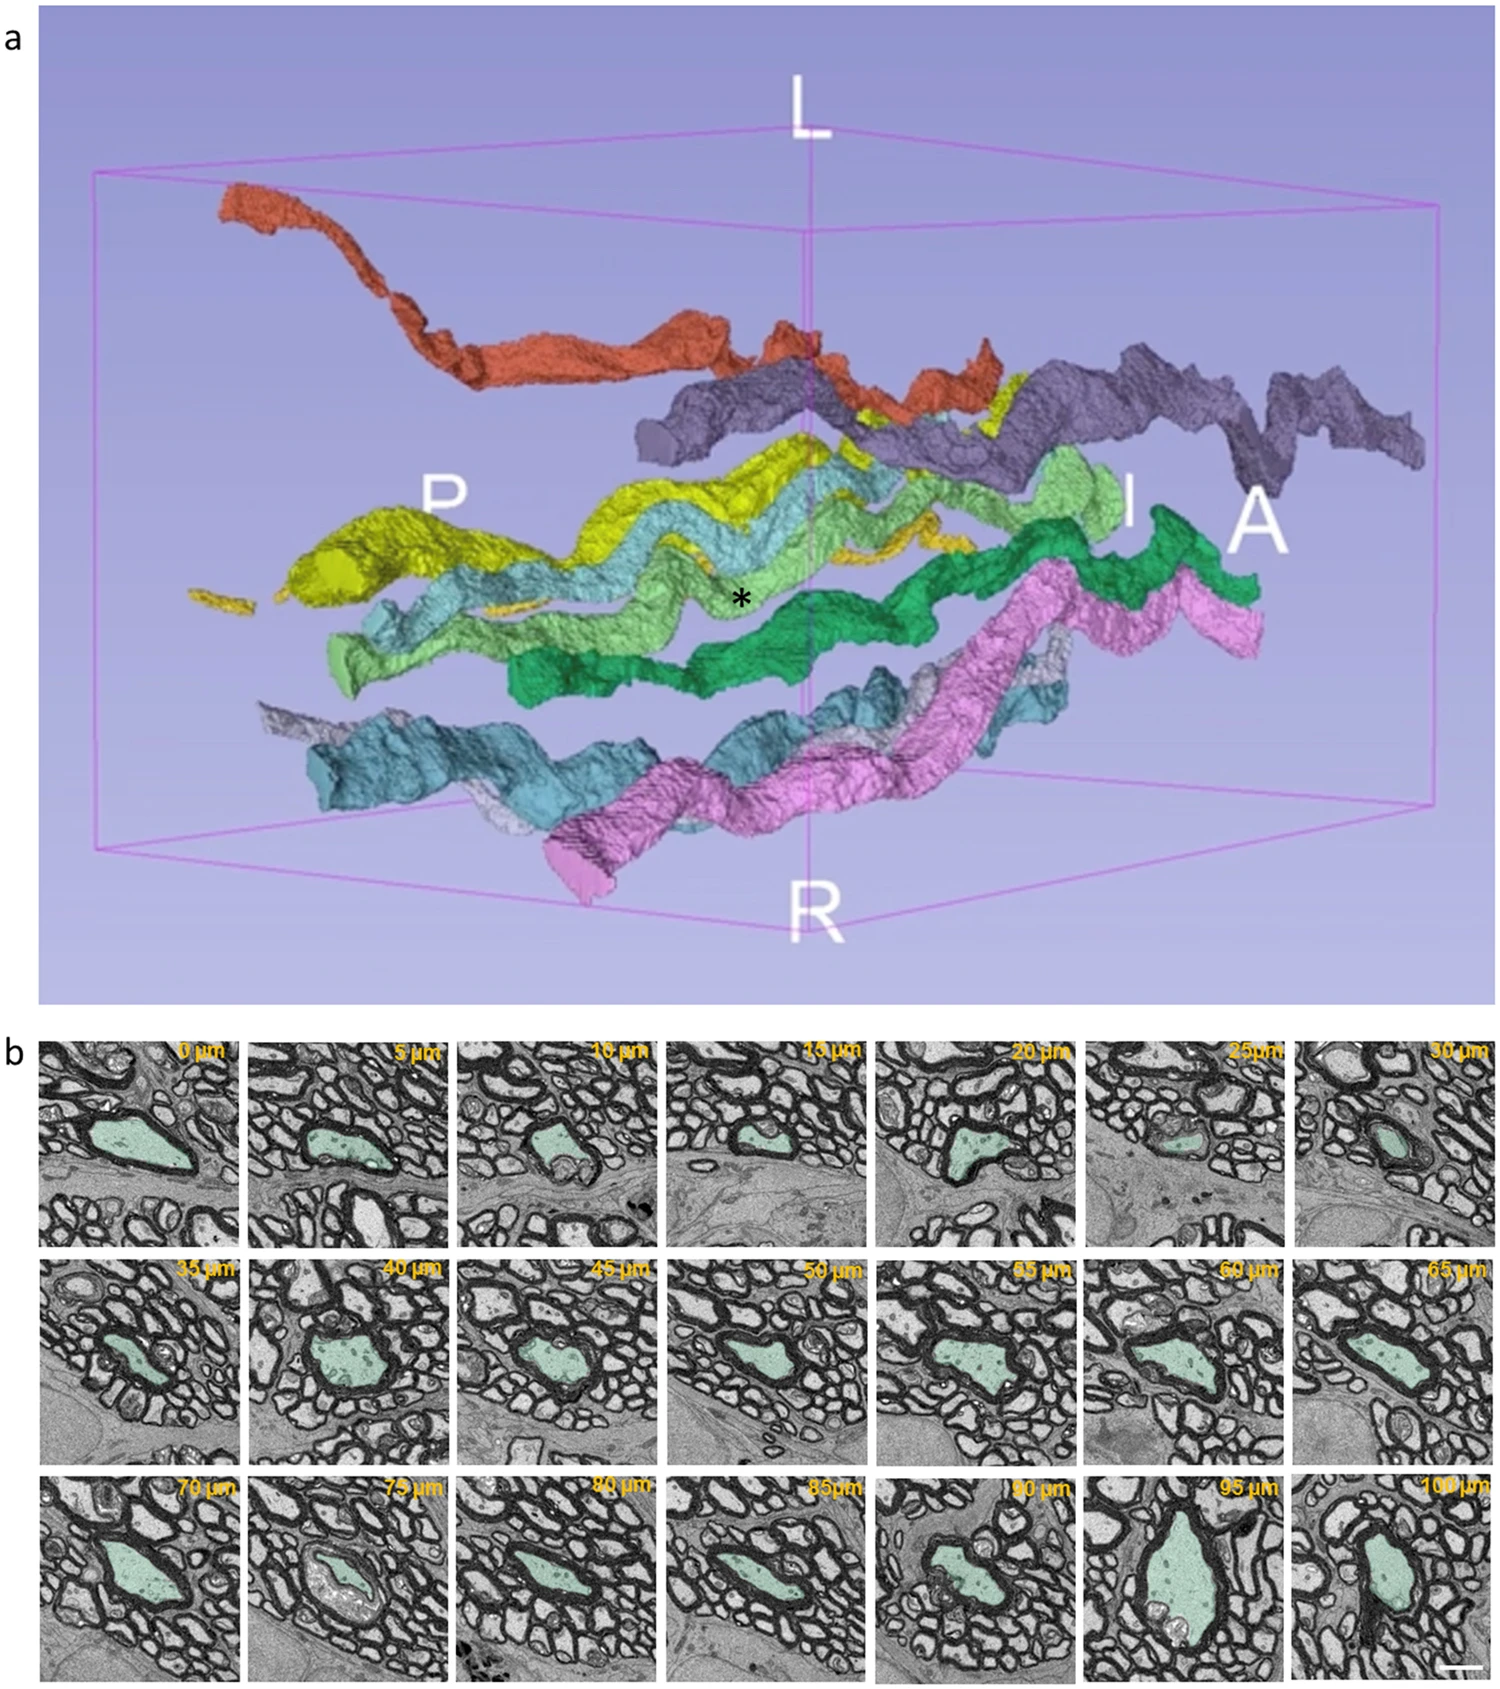
\includegraphics[clip, trim=0.65cm 6.25cm 0.4cm 0.5cm]{gfx/neuroanatomy/nature_3d_em_optical_nerve.png}
	\caption{\dummy{only show a} Three dimensional electron microscopy reveals changing axonal and myelin morphology along normal and partially injured (*, light green) optic nerves. Origin: \cite{Giacci2018} (reative Commons Attribution 4.0 International License).}
% 	\label{fig:brain_sectioning}
\end{figure}
%
\begin{figure}[!t]
	\centering
	\includegraphics{gfx/neuroanatomy/magic.png}
	\caption{Magic. TPFM auto fluorescence nerve fibers. Origin: \cite{Costantini2020}.}
% 	\label{fig:brain_sectioning}
\end{figure}
% 
\begin{figure}[!t]
	\centering
	\tikzset{external/export next=false}
	\begin{tikzpicture}[]   
     \node[inner sep=0pt, anchor = south west] (fig) at (0,0)
       {\includegraphics[width=\textwidth]{gfx/neuroanatomy/NeuralNet-BrainAtlasDotOrg.png}};
     \draw[Orange, ultra thick] (7.65,6.15) ellipse (1 and 0.5);
     \draw[ProcessBlue, ultra thick] (10,4.5) ellipse (2 and 1);
     \draw[white, ultra thick] (0.5,0.5) -- ++ (0:1) node[pos=0.5, above] {\small $\SI{0}{\micro\meter}$};
    \end{tikzpicture}
% 	\includegraphics[width=\textwidth]{gfx/neuroanatomy/NeuralNet-BrainAtlasDotOrg.png}
	\caption{Myelin Staining. human thalamus, sagital section. \textcolor{Orange}{nerve fiber bundles}. \textcolor{ProcessBlue}{neural net}}
% 	\label{fig:brain_sectioning}
\end{figure}
